\subsubsection{Yamauchi \& Takei anelastic shear wave velocity-temperature conversion benchmark}
\label{sec:benchmark-yamauchi-takei}

\textit{This section was contributed by Fred Richards.}

This benchmark tests the implementation of the anelastic shear wave velocity-to-temperature conversion derived by Yamauchi \& Takei~\cite{YT16} based on forced-oscillation experiments conducted at seismic frequencies on polycrystalline borneol. This anelasticity parameterization has been calibrated against a range of observational constraints on upper mantle temperature, attenuation and viscosity structure, using the surface wave tomography model of Priestley et al.~\cite{P12} to constrain shear wave velocity ($V_S$) and the plate model of \cite{McK05} to estimate lithospheric temperature structure. The resulting $V_S$-to-temperature conversion accurately accounts for the strongly non-linear temperature dependence of $V_S$ at near-solidus conditions and is therefore especially useful for initializing models with accurate temperature structure in the upper $\sim$~400 km of the mantle. This benchmark is located in the folder \url{benchmarks/yamauchi_takei_2016_anelasticity}.

\begin{figure}
\begin{center}
  \centering
  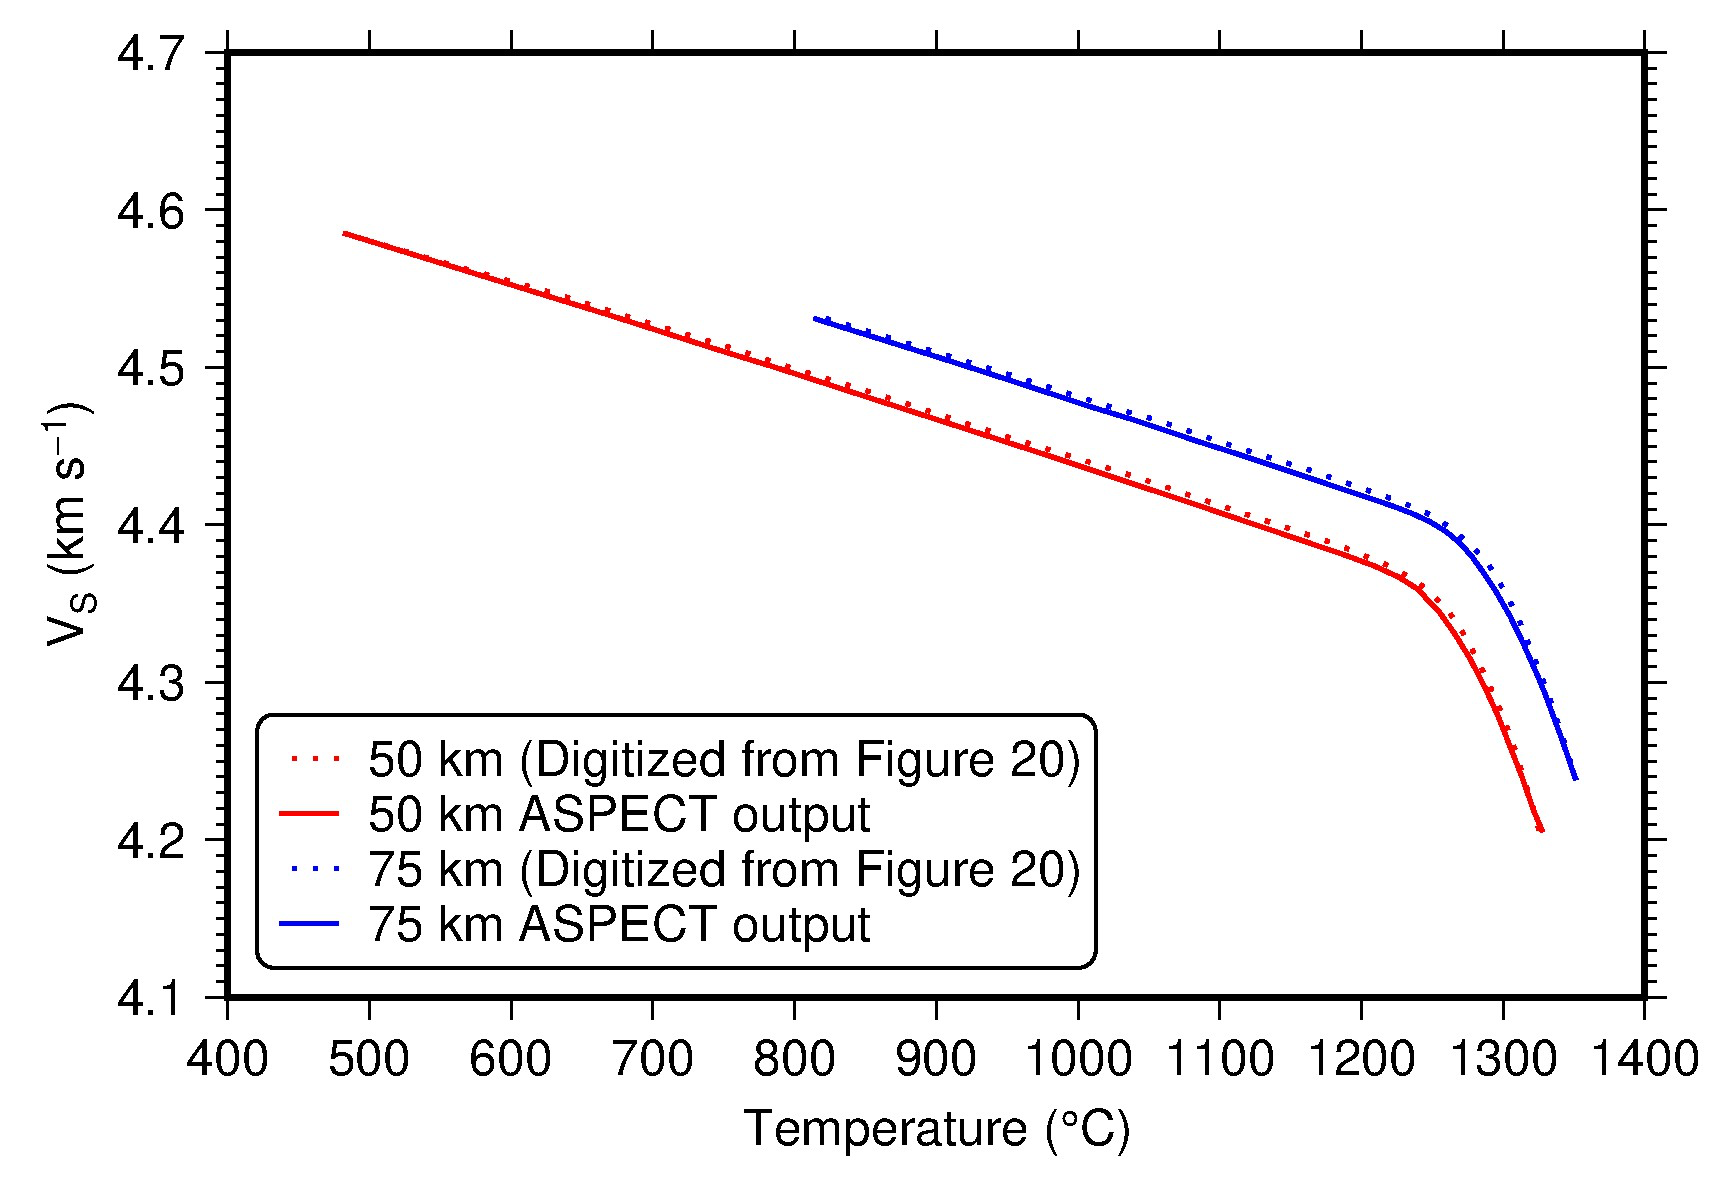
\includegraphics[width=\textwidth]{cookbooks/benchmarks/yamauchi_takei_2016_anelasticity/doc/YT16_benchmark.png}
  \caption{\it $V_S$ as a function of temperature in the oceanic lithosphere. Dotted lines: digitized results from Fig. 20 of Yamauchi \& Takei~\cite{YT16}; solid lines: \aspect{} results; red = 50 km; blue = 75 km. Temperatures are taken from the plate model of McKenzie et al.~\cite{McK05} and $V_{S}$ from the surface wave tomography model of Priestley et al.~\cite{P12}.}
  \label{fig:anelasticity}
\end{center}
\end{figure}

The parameterization of Yamauchi \& Takei~\cite{YT16} defines $V_S$ as
\begin{equation}
V_S = \frac{1}{\sqrt{\rho J_1}} \left( \frac{1+\sqrt{1+(J_2/J_1)^2}}{2}\right)^{-\frac{1}{2}} \simeq \frac{1}{\sqrt{\rho J_1}}
\label{eq:Vs}
\end{equation}
where $\rho$ is the density and $J_1$ and $J_2$ represent real and imaginary components of the complex compliance, $J^*$, which is a quantity describing the sinusoidal strain resulting from the application of a unit sinusoidal stress. $J_1$ represents the strain amplitude in phase with the driving stress, whilst the $J_2$ component is $\frac{\pi}{2}$ out of phase, resulting in dissipation. Density is calculated using the expression
\begin{equation}
\rho (P,T) = \rho_{0}  \left\{ 1 - \left[\alpha(T - T_0)\right] + \frac{P}{K} \right\}
\label{eq:density_P}
\end{equation}
where $\rho_{0} = 3291~\si{kg . m}^{-3}$ and $\alpha = 3.59 \times 10^{-5}~\si{K}^{-1}$ are the density and thermal expansivity corresponding to $T_{0} = 873~\si{K}$, $P$ = pressure and $K = 115.2~\si{GPa}$ is the bulk modulus. $J_1$ and $J_2$ are expressed as
\begin{align}
J_1(\tau_S^{\prime})= & J_U \left[ 1 + \frac{A_B[\tau_S^{\prime}]^{\alpha_B}}{\alpha_B} + \frac{\sqrt{2\pi}}{2} A_P~\sigma_P \left\{ 1-\text{erf}\left(\frac{\ln[\tau_P^{\prime}/\tau_S^{\prime}]}{\sqrt{2}\sigma_P}\right)\right\}\right] \label{eqn:real_compliance} \\
J_2(\tau_S^{\prime}) = & J_U \frac{\pi}{2} \left[ A_B[\tau_S^{\prime}]^{\alpha_B} + A_P~\exp \left(-\frac{\ln^2[\tau_P^{\prime}/\tau_S^{\prime}]}{2\sigma_P^2}\right)\right] + J_U \tau_S^{\prime}
\label{eqn:imaginary_compliance}
\end{align}
where $A_B = 0.664$ and $\alpha_B = 0.38$ represent the amplitude and slope of background stress relaxation and $J_U$ is the unrelaxed compliance. Parameters $A_P$ and $\sigma_P$ represent the amplitude and width of a high frequency relaxation peak superimposed on this background trend such that
\begin{equation}
A_P(T^{\prime}) = \begin{cases}
0.01  &  \text{for }T^{\prime} < 0.91 \\
0.01+0.4(T^{\prime}-0.91) & \text{for }0.91\leq T^{\prime} < 0.96 \\
0.03 & \text{for }0.96\leq T^{\prime} < 1 \\
0.03+\beta(\phi_m) & \text{for }T^{\prime} \geq 1 \\
\end{cases}
\end{equation}
and
\begin{equation}
\sigma_P(T^{\prime}) = \begin{cases}
4  &  \text{for }T^{\prime} < 0.92 \\
4+37.5(T^{\prime}-0.92) & \text{for }0.92\leq T^{\prime} < 1 \\
7& \text{for } T^{\prime} \geq 1 \\
\end{cases}
\end{equation}
where $T^{\prime}$ is the homologous temperature ($\frac{T}{T_{s}}$) with $T$ the temperature and $T_s$ the solidus temperature, both in Kelvin. $\phi_m$ is the melt fraction and $\beta(\phi_m)$ describes the direct poroelastic effect of melt (assumed to be negligible under upper mantle conditions). For this case, $J_U$ is the inverse of the unrelaxed shear modulus, $\mu_{U}(P,T)$, such that
\begin{equation}
J_{U}(P,T)^{-1} = \mu_U(P,T) = \mu_U^0 + \frac{\partial{\mu_U}}{\partial{T}}(T -T_0)+ \frac{\partial{\mu_U}}{\partial{P}}(P-P_0)
\end{equation}
where $\mu_U^0$ is the unrelaxed shear modulus at surface pressure-temperature conditions, the differential terms are assumed to be constant and the pressure, $P$, in GPa is linearly related to the depth, $z$, in km by $\frac{z}{30}$. The normalised shear wave period, $\tau_S^{\prime}$, in Equations~\eqref{eqn:real_compliance} and \eqref{eqn:imaginary_compliance} is equal to $\frac{\tau_S}{2\pi\tau_M}$, where $\tau_S = 100~\si{s}$ is the shear wave period and $\tau_M = \frac{\eta}{\mu_U}$ is the normalised Maxwell relaxation timescale. $\tau_P^{\prime}$ represents the normalised shear-wave period associated with the centre of the high frequency relaxation peak, assumed to be $6 \times 10^{-5}$. The shear viscosity, $\eta$, is
\begin{equation}
\eta = \eta_r \left(\frac{d}{d_r}\right)^{m} \exp \left[ \frac{E_a}{R}\left(\frac{1}{T}-\frac{1}{T_r}\right) \right] \exp \left[ \frac{V_a}{R}\left(\frac{P}{T}-\frac{P_r}{T_r}\right) \right] A_{\eta}
\label{eq:eta}
\end{equation}
where $d$ is the grain size, $m$ the grain size exponent (assumed to be 3), $R$ the gas constant, $E_a$ the activation energy and $V_a$ the activation volume. Subscripts $[X]_r$ refer to reference values, assumed to be $d_r = d = 1~\si{mm}$, $P_r = 1.5~\si{GPa}$ and $T_r = 1473~\si{K}$ for the upper mantle. $A_{\eta}$ represents the extra reduction of viscosity due to an increase in $E_a$ near the solidus, expressed as
\begin{equation}
A_\eta(T^{\prime}) =
\begin{cases}
1  & \text{for } T^{\prime} < T^{\prime}_{\eta} \\
\exp \left[-\frac{(T^{\prime}-T^{\prime}_{\eta})}{(T^{\prime}-T^{\prime}T^{\prime}_{\eta})} \ln(\gamma)\right]& \text{for }T^{\prime}_{\eta} \leq T^{\prime} < 1 \\
\gamma^{-1} \exp(\lambda\phi) & \text{for }T^{\prime} \geq 1\\
\end{cases}
\end{equation}
where $T^{\prime}_\eta$ is the homologous temperature above which activation energy becomes $E_a + \Delta E_a$, and $\gamma = 5$ is the factor of additional reduction. $\lambda\phi$ describes the direct effect of melt on viscosity, assumed to be negligible here. The solidus temperature, $T_s$, is fixed to a value of 1599~K at 50~km equivalent to a dry peridotite solidus \cite{Hirsch2000} and linearly increases below this depth according to
\begin{equation}
T_{s}(z) = 1599 + \frac {\partial T_s}{\partial z} (z - 50000)
\label{eq:Ts}
\end{equation}
where $\frac {\partial T_s}{\partial z}$ is the solidus gradient.

In this benchmark, a 2D input ASCII file containing $V_S$ specified at 50 and 75 km depth is read in and converted to temperature using an initial temperature model that implements the $V_{S}(P,T)$ formulation detailed above. The default parameters governing the relationship between $V_S$ and temperature are set to the values calibrated by Yamauchi \& Takei~\cite{YT16}, where $\mu_U^0 = 72.45~\si{GPa}$, $\frac{\partial{\mu_U}}{\partial{T}} = -0.01094~\si{GPa . K}^{-1}$, $\frac{\partial{\mu_U}}{\partial{P}} = 1.987$,  $\eta_r = 6.22 \times 10^{21}~\si{Pa . s}$, $E_a = 452.5~\si{kJ . mol}^{-1}$, $V_a = 7.913 \times 10^{-6}~\si{m}^{3}~\si{mol}^{-1}$ and $\frac{\partial T_s}{\partial z} = 1.018~\si{K . km}^{-1}$. As $V_S$ is a complex function of temperature, a Brent minimization algorithm is used to find optimal values. Fig.~\ref{fig:anelasticity} shows that the \aspect{} implementation of this parameterization can accurately recreate the results shown by Yamauchi \& Takei~\cite{YT16} in their Fig. 20.

The parameter file and initial temperature model for this benchmark can be found at \url{benchmarks/yamauchi_takei_2016_anelasticity/yamauchi_takei_2016_anelasticity.prm} and \url{benchmarks/yamauchi_takei_2016_anelasticity/anelasticity_temperature.cc}. Code to recreate  Fig.~\ref{fig:anelasticity}  is provided in \url{benchmarks/yamauchi_takei_2016_anelasticity/plot_output}.
